\documentclass[conference]{IEEEtran}
\IEEEoverridecommandlockouts
% The preceding line is only needed to identify funding in the first footnote. If that is unneeded, please comment it out.
\usepackage{cite}
\usepackage{amsmath,amssymb,amsfonts}
\usepackage{algorithmic}
\usepackage{graphicx}
\usepackage{textcomp}
\usepackage{xcolor}
\def\BibTeX{{\rm B\kern-.05em{\sc i\kern-.025em b}\kern-.08em
    T\kern-.1667em\lower.7ex\hbox{E}\kern-.125emX}}
\renewcommand\IEEEkeywordsname{Keywords}

\begin{document}

\title{ Implementation of Grover’s Algorithm based on
	Quantum Reservoir Computing  \\

}
\author{\IEEEauthorblockN{Shivani Mehta}
	\IEEEauthorblockA{\textit{Department of ECE,} \\
		\textit{IIITDM Kancheepuram,}\\
		Chennai-600127, India.\\
		ec22m2002@iiitdm.ac.in}
	\and
	\IEEEauthorblockN{Sajja Jyothikrishna}
	\IEEEauthorblockA{\textit{Department of ECE,} \\
		\textit{IIITDM Kancheepuram,}\\
		Chennai-600127, India. \\
		ec21b1022@iiitdm.ac.in}
	\and
	\IEEEauthorblockN{V.Praveen Bhallamudi}
	\IEEEauthorblockA{\textit{Department of Physics,} \\
		\textit{IIITDM Kancheepuram,}\\
		Chennai-600036, India. \\
		praveen.bhallamudi@iitm.ac.in}
	\and
	\IEEEauthorblockN{Sumanth Arige}
	\IEEEauthorblockA{\textit{Department of ECE,} \\
		\textit{IIITDM Kancheepuram,}\\
		Chennai-600127, India. \\
		edm20d010@iiitdm.ac.in}
	\and

	\IEEEauthorblockN{ Tejendra Dixit, $Member, IEEE$}
	\IEEEauthorblockA{\textit{Department of ECE,} \\
		\textit{IIITDM Kancheepuram,}\\
		Chennai-600127, India. \\
		tdixit@iiitdm.ac.in}
}

\maketitle

\begin{abstract}
	Quantum computing represents the leading edge of
	computational technology, leveraging the principles of quantum
	mechanics to execute targeted computations much faster than
	classical computers. In contrast to classical bits, which are limited
	to representing either 0 or 1, qubits, or quantum bits, exhibit
	the extraordinary property of superposition. This distinctive
	characteristic enables qubits to simultaneously occupy multiple
	states, empowering quantum computers to explore numerous
	potential solutions to a problem concurrently. This feature
	makes quantum computing particularly potent for specific tasks.
	Recent research endeavors have been sparked by the potential
	of advanced quantum computing technology, leading to the
	creation of simulations of quantum computers using classical
	hardware. Grover’s quantum search algorithm serves as a notable
	illustration of quantum computing application, enabling quantum
	computers to conduct a database search within an unsorted array
	with a quadratic speedup in time efficiency compared to classical
	computers. This document presents the quantum Grover search
	algorithm and its application through 5-qubit quantum circuits,
	as well as a design framework to simplify the creation of an
	oracle for a greater number of qubits.
\end{abstract}

\begin{IEEEkeywords}
	Quantum computation, Qubits, Oracle, Grover’s
	algorithm, IBM Qiskit.
\end{IEEEkeywords}

\section{Introduction}
The exploration of quantum computing [1][2] falls within
the realm of quantum information science, which revolves
around the fundamental principles of storing and manipulating
information. In this work, we delved into quantum computing,
acquiring a comprehensive understanding of quantum bits
and their properties, as well as leveraging these properties
to tackle problems. We familiarized ourselves with quantum
gates and their operations on qubits, simulating all the fundamental quantum gates [3][4]. Additionally, we delved into the
Grover search algorithm and implemented quantum gates for
Grover operations. Quantum computers exhibit significantly
faster speeds compared to classical computers [5][6]. In the
case of an unsorted dataset with size N, classical computers
usually demand O(N) operations, whereas Grover’s algorithm
accomplishes this task optimally in O($\sqrt{N}$) operations.
\\
We
executed the algorithm using Qiskit, an IBM tool for computing quantum circuits, and conducted simulations for the
Grover algorithm [7], presenting the results graphically with
the probability of obtaining the correct output.

Within Grover’s quantum search algorithm, a network with
n qubits harbors $ 2^{n} $ = N states, with each state bearing a
probability of $ 1/N $ for discovery. Consequently, the amplitude
of each state is $ 1/\sqrt{N} $
. Conversely, classical systems tackling the
same problem necessitate a maximum of O(N) trials.
\section{Background and Methodology}

The Grover search algorithm, conceived by Lov Grover
in 1996, stands as a quantum computing method offering
a quadratic acceleration compared to classical counterparts,
particularly for solving unstructured search problems [8]. It
has gained renown for its proficiency in searching through
unsorted databases, but its utility extends to a spectrum
of tasks, encompassing cryptographic problem-solving and
quantum system simulation. This can speed up a search
problem quadratically. For N number of unsorted data classical
computer require O (N) operations Whereas Grover is optimal
and can do this in O($ \sqrt{N} $) operation. The following provides
a synopsis of the workings of the Grover search algorithm [9]:
\subsection{Initialisation}
Commencing the process involves establishing a superposition of all conceivable states. For instance, when seeking an
item in a database housing N item, quantum parallelism is
harnessed to generate a superposition of all N states as shown
in Fig.1. Achieving this involves a sequence of quantum gate
operations.

\begin{figure}[htbp]
	\centerline{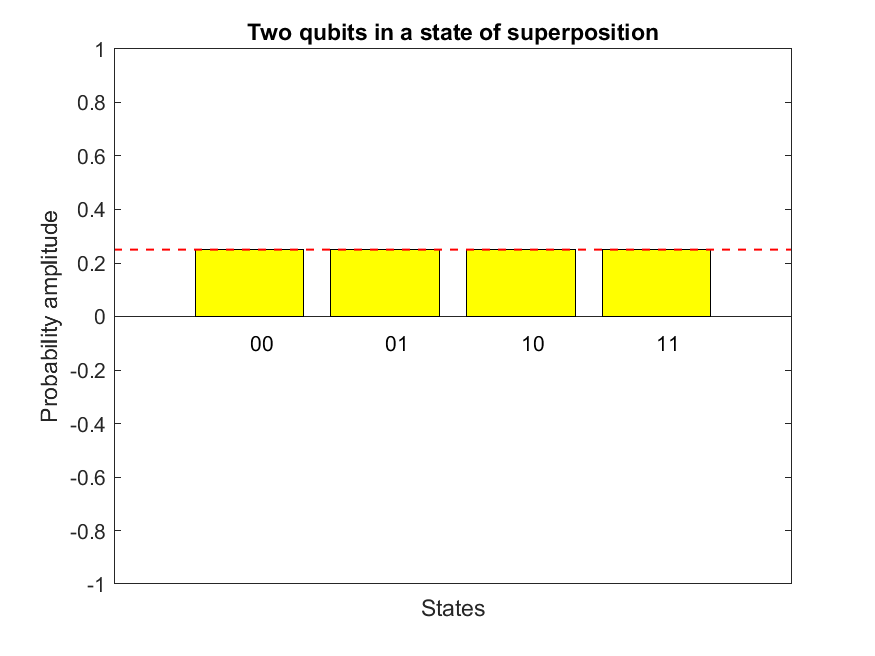
\includegraphics[width=9cm,height=10cm,keepaspectratio]{fig1.png}}
	\caption{Superposition of 2 qubits}
	\label{fig}
\end{figure}

\subsection{Oracle Function}
Grover’s algorithm hinges on the application of an oracle
function, often denoted as \textbf{"$ U_f $"}. This oracle acts to mark
the target state(s) by inverting their sign. For instance, if the
objective is to locate a specific item in a database, the oracle
would negate the amplitude corresponding to the target item.
In Fig. 2, it is graphically shown the oracle function flipping
the correct target.

\begin{figure}[htbp]
	\centerline{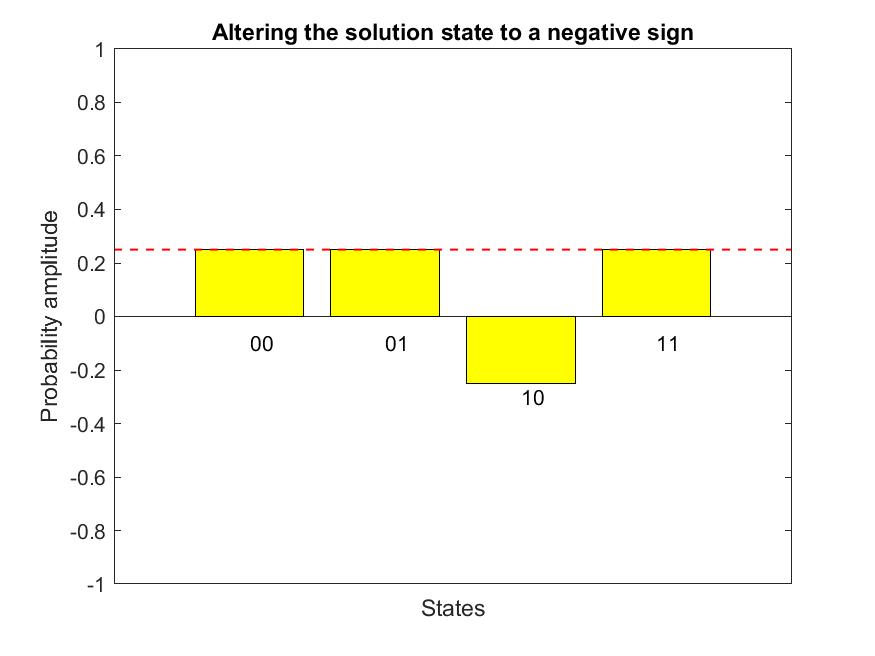
\includegraphics[width=9cm,height=10cm,keepaspectratio]{fig2.png}}
	\caption{Altering the sign of solution state(10)}
	\label{fig}
\end{figure}

\subsection{Amplitude Amplification}
The core of the Grover algorithm is the process of amplitude
amplification, which entails two central maneuvers:
\begin{itemize}
	\item \textbf{Inversion around the Mean}: During this stage, the amplitudes are mirrored around their average value, thus  boosting the amplitude of the desired state(s) while reducing the amplitudes of the non-desired states.
	\item \textbf{Grover diffusion operator}: In this step, the amplitudes
	      of the target state(s) are further augmented through the
	      application of a suite of quantum gates [10].

\end{itemize}
After acting of Grover diffusion operator, the final output will
have amplified magnitude as shown in Fig. 3.
\subsection{Reiteration}
Step. 2 and step. 3 are iterated approximately $ \sqrt{N} $ times
to maximize the likelihood of detecting the correct state. This
number of iterations ensures that the probability of identifying
the correct state approaches near certainty.

\begin{figure}[htbp]
	\centerline{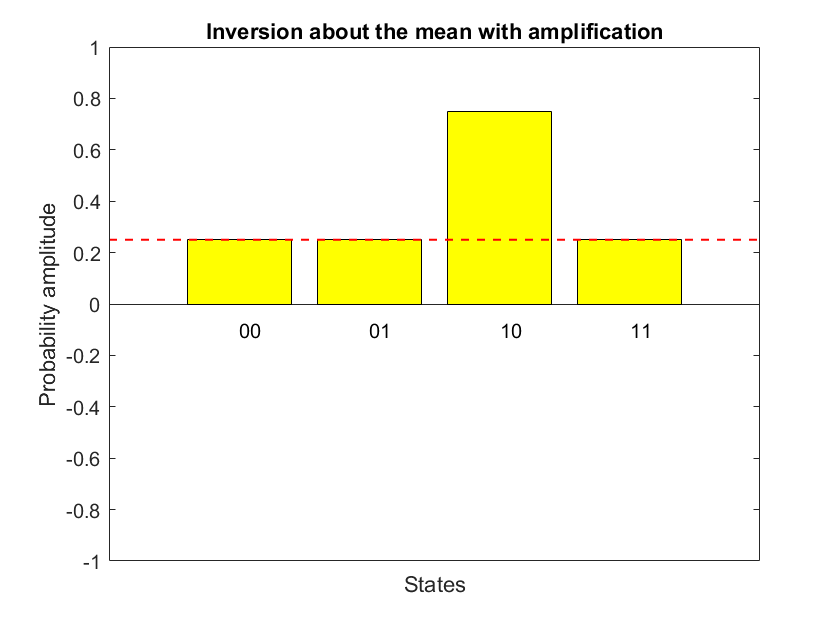
\includegraphics[width=9cm,height=10cm,keepaspectratio]{fig3.png}}
	\caption{Inversion about the mean with amplification.}
	\label{fig}
\end{figure}

\subsection{ Measurement}
Ultimately, the quantum state is subjected to measurement.
The target state is discerned with notably higher probability in comparison to the non-target state.

\section{ CONSTRUCTION OF ORACLE AND DIFFUSION
  OPERATOR}
The Grover iteration, also known as the Grover operator,
constitutes a crucial component of the quantum search process.
It encompasses two distinct phases. At the outset, the oracle
function modifies the phase of a single amplitude within a
marked state. Upon completion of this phase, referred to as
the diffusion layer, the indicated state amplitude is flipped.
Consequently, while the amplitudes of the other states remain
unchanged, the target state assumes an inverted state, resulting
in a notable increase in its amplitude and a slight decrease in
the amplitudes of the other states. The block diagram of Grover
iteration circuit is shown below in Fig. 4.

\begin{figure}[htbp]
	\centerline{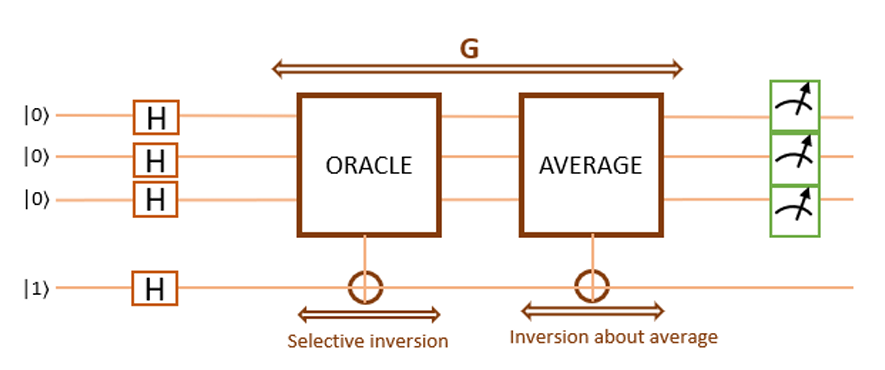
\includegraphics[width=9cm,height=10cm,keepaspectratio]{fig4.png}}
	\caption{Grover Iteration circuit}
	\label{fig}
\end{figure}

\subsection{ORACLE}
An oracle, defined as a medium or agency for divine
revelation, particularly noted in ancient Greece, also refers
to a person possessing great wisdom or a wise utterance. In
quantum computing, a quantum oracle [11] is a computational
component that furnishes data pertinent to the particular prob
lem or task undergoing processing by the quantum algorithm.
The quantum oracle performs a bit-flip on the oracle qubit when the input corresponds to a valid solution.The functionality of the oracle operates on principles rather than mystical
properties.Through the abstraction of the problem using an
oracle,we can focus on solving the problem without being
constrained by its specific details.This quantum algorithm is
crafted to determine the input value x* for a function F(x),
where F(x*) = 1 and F(x) = 0 for all other values of x.

\subsection{DIFFUSION OPERATOR}
The diffusion operation can be realized through the sequence:HX+Oracle+XH. In this scenario, H symbolizes
the Hadamard transform,while X represents the Pauli-X gate.
This sequence effectively flips the amplitudes around their
mean value. Simulation of Hadamard gate, Pauli-x gate and
Zero phase shift gate in Qiskit are shown in Fig.5,Fig.6and
Fig.7respectively[12].

\section{CIRCUIT IMPLEMENTATION AND RESULTS}
Grover’s oracle is developed and Grover's algorithm is implemented using Q-simulator from
Qiskit.

\subsection{Simulation Results}
Simulation results for 3-qubit, 4-qubit and 5-qubit Grover
search algorithm are shown in Fig. 11, Fig. 12 and Fig.
13 respectively. In 1,024 measurements with the ibmqx4,
the outcome x = (110) was observed 966 times (Fig. 11),
corresponding to a probability of 94.33 percent. In 1,024
measurements with the ibmqx4, the outcome x = (1011) was
observed 987 times (Fig. 12), corresponding to a probability
of 96.38 percent. In 1,024 measurements with the ibmqx4,
the outcome x = (11010) was observed 1023 times (Fig. 13),
corresponding to a probability of 99.90 percent

\section{CONCLUSION}
In summary, quantum computing presents an intriguing
pathway for addressing intricate problems that surpass the capabilities of classical computers. Qiskit’s quantum computing
platform offers a sturdy framework for creating, simulating,
and executing quantum algorithms. In contrast to classical
search algorithms, which require O(N) operations for N
items, Grover’s algorithm achieves this task in approximately
O($\sqrt{N} $) operations. Initially, we replicated IBM’s proposed
Grover search algorithm for 3 qubits. To enhance fidelity, we
modified the design of the Oracle and Diffusion operators by
incorporating auxiliary qubits. However, this led to increased
circuit complexity due to a larger number of gates. The
experiments were conducted using the IBM Q-simulator. The
results indicate that the scalable Grover’s search technique
proposed can potentially be employed in future quantum
systems for a wide range of large-scale applications. Since
the diffusion process incorporates the Oracle (HX + Oracle +
XH), iteratively running the Oracle circuit multiple times complicates the quantum circuit and decreases its effectiveness.
Nonetheless, by designing the Oracle as a subroutine, we can
leverage the advantages of reusability. This strategy mitigates
potential manual mistakes and streamlines the process by
eliminating the necessity of re-executing all the gates, with
IBM Q providing assistance for subroutines. Subsequently,
using this 5-qubit setup as a benchmark, the algorithm will
be extended to n-qubits.


\begin{thebibliography}{00}

	\bibitem{b1}  C. P. Williams, “Introduction,” Texts in Computer Science, pp. 3–49,
	2011.

	\bibitem{b2}  T. D. Ladd, F. Jelezko, R. Laflamme, Y. Nakamura, C. Monroe, and
	J. L. O’Brien, “Quantum computers,” Nature, vol. 464, no. 7285, pp.
	45–53, Mar. 2010.

	\bibitem{b3} “Quantum Computing: Fundamentals, Implementations and Applications” — IEEE Journals Magazine — IEEE Xplore, ieeexplore.ieee.org.

	\bibitem{b4} D. P. DiVincenzo, “The Physical Implementation of Quantum Computation,” Fortschritte der Physik, vol. 48, no. 9–11, pp. 771–783, Sep.
	2000.
	\bibitem{b5}  D. Bacon and W. van Dam, “Recent progress in quantum algorithms,”
	Communications of the ACM, vol. 53, no. 2, pp. 84–93, Feb. 2010.

	\bibitem{b6}  N. C¸elik and ¨ O. Bing¨ ol, “Analysis of Grover’s quantum search algorithm
	on a classical computer: Identifying opportunities for improvement,”
	Sigma Journal of Engineering and Natural Sciences, vol. 42, no. 6, 2024.

	\bibitem{b7} “Learn Quantum Computing with Python and IBM Quantum Experience: A hands-on introduction to quantum computing and writing your own quantum programs with Python- Robert Loredo- Libro in linguainglese- Packt Publishing Limited- — IBS,” www.ibs.it.

	\bibitem{b8}  L. K. Grover, “A fast quantum mechanical algorithm for database search,” arXiv:quant-ph/9605043, Nov. 1996.

	\bibitem{b9} A. J. et al., “Quantum Algorithm Implementations for Beginners,” arXiv:1804.03719 [quant-ph], Mar. 2020.

	\bibitem{b10}  “Quantum Game Simulator, Using the Circuit Model of Quantum — IEEE Conference Publication — IEEE Xplore,” ieeexplore.ieee.org.

	\bibitem{b11}  C. B. Pronin and A. V. Ostroukh, “Developing Mathematical Oracle
	Functions for Grover Quantum Search Algorithm,” arXiv.org, Sep. 03,
	2021.

	\bibitem{b12} R. L. Singleton Jr, M. L. Rogers, and D. L. Ostby, “Grover’s Algorithm
	with Diffusion and Amplitude Steering,” arXiv.org, Oct. 21, 2021.

	\bibitem{b13}  D. J. Shepherd, “On the Role of Hadamard Gates in Quantum Circuits,”
	Quantum Information Processing, vol. 5, no. 3, pp. 161–177, May 2006.

	\bibitem{b14} A. Mandviwalla, K. Ohshiro, and B. Ji, “Implementing Grover’s Algorithm on the IBM Quantum Computers.”

	\bibitem{b15}  D. Reddy Vemula, D. Konar, S. Satheesan, M. Kalidasu, and A. Cangi,
	“A Scalable 5,6-Qubit Grover’s Quantum Search Algorithm.”.
\end{thebibliography}

\end{document}
